\documentclass[12pt,oneside,notitlepage,abstracton,a4paper]{scrartcl}
\usepackage{epsfig,scrpage2,graphicx}
\usepackage{epstopdf}
\usepackage{psfrag}
\usepackage[framed,numbered,autolinebreaks,useliterate]{mcode}

\usepackage{colortbl}

\definecolor{maroon}{cmyk}{0,0.87,0.68,0.32}

\newcommand{\gray}{\rowcolor[gray]{.90}}

\newtheorem{theorem}{\textbf{Theorem}}[section]
\newtheorem{proposition}{\textbf{Proposition}}[section]
\newtheorem{corollary}{\textbf{Corollary}}[section]
\newtheorem{definition}{\textbf{Definition}}[section]
\newtheorem{fact}{\textbf{Fact}}[section]
\newtheorem{lemma}{\textbf{Lemma}}[section]
\newtheorem{assumption}{\textbf{Assumption}}[section]
\newtheorem{problem}{\textbf{Problem}}[section]
\newtheorem{remark}{\textbf{Remark}}[section]
\newtheorem{example}{\textbf{Example}}[section]
\newtheorem{property}[section]{\textbf{Property}}

\newcommand{\bc}{\begin{center}}
\newcommand{\ec}{\end{center}}
\newcommand{\bt}{\begin{tabular}}
\newcommand{\et}{\end{tabular}}

\newcommand{\JR}[1]{\textcolor{red}{#1}}
 
\newcommand\Ltwo{\ensuremath{\mathcal{L}_2}}
\newcommand\real{\ensuremath{\mathbb R}}
\newcommand\dz{\ensuremath{\mbox{dz}}}
\newcommand\sat{\ensuremath{\mbox{sat}}}
\newcommand\diag{\ensuremath{\mbox{diag}}}
\newcommand\calq{\ensuremath{\mathcal Q}}
\newcommand{\smallmat}[1]{\left[ \begin{smallmatrix}#1\end{smallmatrix} \right]}
 
%Commands
\newcommand{\bbar}[1]{\bar{\bar{#1}}}
\newcommand{\ba}[1]{\begin{array}{#1}}
\newcommand{\ea}{\end{array}}
\newcommand{\matrice}[2]{\left [ \ba{#1} #2 \ea \right ]}
\newcommand{\beq}{\begin{equation}}
\newcommand{\eeq}{\end{equation}}
\newcommand{\beqa}{\begin{eqnarray}}
\newcommand{\eeqa}{\end{eqnarray}}
\newcommand{\bns}{\begin{normalsize}}
\newcommand{\ens}{\end{normalsize}}
\newcommand{\bss}{\begin{small}}
\newcommand{\ess}{\end{small}}
\newcommand{\bfs}{\begin{footnotesize}}
\newcommand{\efs}{\end{footnotesize}}
\newcommand{\bsz}{\begin{scriptsize}}
\newcommand{\esz}{\end{scriptsize}}
\newcommand{\bsm}{\begin{smallmatrix}}
\newcommand{\esm}{\end{smallmatrix}}
\newcommand{\zeros}[2]{\mathbf{0}_{#1 \times #2}}
\newcommand{\interior}[1]{\stackrel{\circ}{#1}}
\newcommand{\mycaption}[1]{\caption{\baselineskip=15pt \protect{#1}}}
\newcommand{\giu}[1]{\vspace*{#1mm}}
 
\setcounter{secnumdepth}{3}

\setlength{\parindent}{0em}
\setlength{\parskip}{0ex plus0.5ex minus0ex}
\pagestyle{scrheadings}
\bibliographystyle{unsrt}   

\renewcommand{\headfont}{\normalfont}

\cfoot{\pagemark}

%\titlehead{EUDET-Memo-2010-04}
 
%\subject{\includegraphics[scale=0.4]{pics/anemone}}
%\subject{\includegraphics[scale=0.4]{pics/logo.eps}}
%bb=0 0 179 200,
 
\title{\Huge  \textcolor{blue}{EquiSim\\User's Manual}} 
\author{\normalsize Toufik BENTALEB}
\subject{\normalsize Univ Lyon, Universit\'e Claude Bernard Lyon 1, Univ Gustave Eiffel, IFSTTAR, LBMC UMR\_T9406}
\date{\normalsize \today}

\begin{document}

\maketitle

\vspace{5em}
\begin{abstract}
\noindent
This manual is intended to help users to run and to know how and where they can perform any modification in the EquiSim software tool. This software tool was developed to allow human balance prevention and recovery to be performed using MATLAB and using linear model predictive control (LMPC) algorithm. A “Quick Start” approach to using this software will be presented, along with a detailed section containing full explanations and examples for using this tool.
\end{abstract}
  
\newpage
\tableofcontents
\newpage 

\section{Introduction}
\label{intro}
The aim of this document is to help users to use the MATLAB software tool for human/robot balance prevention and recovery. It is intended to provide all necessary information in a simple way. A ''Quick Start'' approach to using this tool will be presented, along with a detailed. The EquiSim user's manual contains a thorough description of all files in the software tool.

%{\color{red} 
%In \textbf{Section~\ref{System}} a short description of the system requirements to run the software.  
%\textbf{Section~\ref{How}} is explained how files of the software are organised.  
%\textbf{Section~\ref{Quick}} is explained how to run the software.
%\textbf{Section~\ref{Getting}} gives a description of the MATLAB scripts.
%The implementation of MPC control in Simulink and an example are  discussed in \textbf{Section~\ref{Model}}.
%}
   
\section{System Requirements} \label{System}
In order to get the code to execute properly, the following programs are required:
\begin{enumerate}
  \item The program has been developed for use in the MATLAB environment and it is running perfectly on \textbf{\texttt{MATLAB 2017b}} (\textbf{\texttt{MATLAB 9.03.0}}).    
  \item To solve the quadratic programming problem using \textbf{\texttt{quadprog}} function the \textbf{\texttt{OPTIMIZATION TOOLBOX}} is required.
  %\item The \textbf{Aerospace Blockset} from \textbf{MATLAB} is required.
\end{enumerate}

\section{How files are organised} \label{How}
The folder \textbf{\texttt{EquiSim\_folder}} contains all files necessary of the software tool, were divided into many categories: 
\begin{itemize}
	  \item  The main Matlab script file \textbf{\texttt{main\_EquiSim.m}} to run the program. 
	  \item  The folder \textbf{\texttt{core\_test}} contains \textbf{\texttt{classdef}}, \textbf{\texttt{function}}, and \textbf{\texttt{script}} folders because the software was built using Object-Oriented (OO) techniques. 
	  \item  The folder \textbf{\texttt{core\_MPC}} contains \textbf{\texttt{classdef}}, \textbf{\texttt{function}}, and \textbf{\texttt{script}} folders. 
	  \item  The folder \textbf{\texttt{core\_physical\_model}} contains \textbf{\texttt{classdef}}, \textbf{\texttt{function}}, and \textbf{\texttt{script}} folders. 
	  \item  The folder \textbf{\texttt{results}} contains results graphs, for the test performed, in format of  \textbf{\texttt{*.JPG}}, \textbf{\texttt{*.EPS}} and \textbf{\texttt{*.PDF}}. 
\end{itemize}

\nopagebreak
\pagebreak 
\section{Control scheme}
 The feedback loop used to simulate the balance recovery is shown in the Fig.~\ref{fig:control_scheme}. When you run the main function \textbf{\texttt{main\_EquiSim}}, the software starts to add all subfolders to matlab path and prepare storage files after that, it runs \textbf{\texttt{classdef\_create\_experiment}} which is shown in the scheme below by \textit{\texttt{Desired final states}}. After creating the human model (using \textit{\texttt{script\_constant.m}}), and the experiment steps (using \textbf{\texttt{classdef\_create\_experiment}}), the inputs of a MPC iteration are created. The \textit{\texttt{Mechanical Model}} is the physical model of the human, in the code we use \textbf{\texttt{classdef\_physical\_model}} to run it. To add the disturbance to the physical model just uncomment \textbf{\texttt{physical\_model\_storage.add\_storage\_sensors}}  and comment \textbf{\texttt{physical\_model\_storage.add\_storage}}. The same for the delay in the model (the \textit{\texttt{Sensors}} in the scheme) you need just give the neural time delay (\textbf{\texttt{neural\_time\_delay}}) and uncomment \textbf{\texttt{sensor\_dynamics.sensor\_dynamics\_iteration}}.        

\begin{figure}[ht]   % I have to describe this part  
\centering 
\psfrag{mm}[Bc][Bc][1]{\footnotesize \textbf{Mechanical Model}}   
\psfrag{in}[Bc][Bc][1]{\footnotesize 3D inverted pendulum}
\psfrag{ds}[Bc][Bc][1]{\footnotesize Disturbance}
\psfrag{vm}[Bc][Bc][1]{\footnotesize Movement}
\psfrag{op}[Bc][Bc][1]{\footnotesize Optimiser}   
\psfrag{cf}[Bc][Bc][1]{\footnotesize Cost function} 
\psfrag{cs}[Bc][Bc][1]{\footnotesize +constraints} 
\psfrag{im}[Bc][Bc][1]{\footnotesize Internal Model}  
\psfrag{lip}[Bc][Bc][1]{\footnotesize (LIPM)}  
\psfrag{dis}[Bc][Bc][1]{\footnotesize Desired final states}  
\psfrag{mpc}[Bc][Bc][1]{\footnotesize \textbf{Model Predictive Controller}} 
\psfrag{sens}[Bc][Bc][1]{\footnotesize \textbf{Sensors}}   
\psfrag{s}[Bc][Bc][2]{\footnotesize \textbf{$\sum$}}    
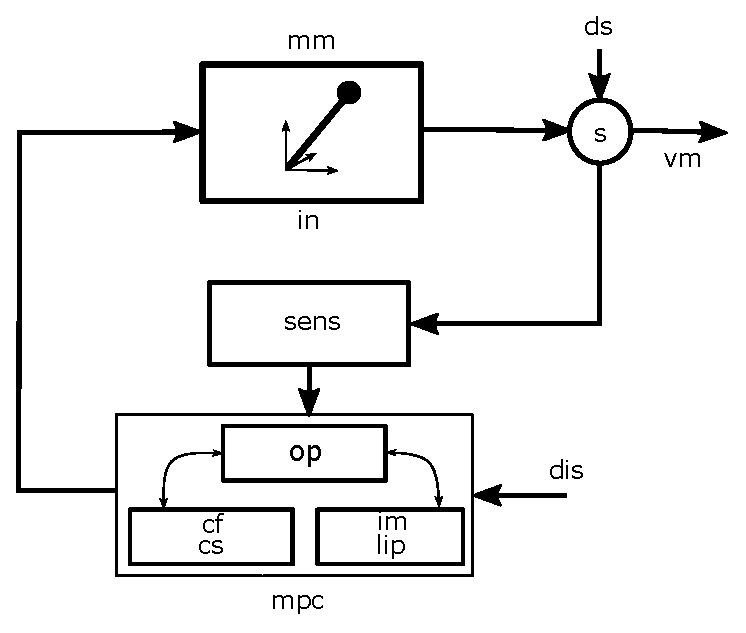
\includegraphics[angle=0,width=.7\columnwidth]{images/control_scheme/control_scheme.eps}
\caption{Flow diagram of the human balance recovery}\label{fig:control_scheme}
\end{figure} 

\clearpage
\newpage
\section{Getting started with software}\label{Getting}
This section will take you through one example in order to get you started with 
the MATLAB software tool for human/robot balance prevention and recovery.

%\pagebreak 
\subsection{The main function}
 The m-script \textbf{\texttt{main\_EquiSim.m}} is the only file visible in the folder \textbf{\texttt{EquiSim\_folder}} to run the software, and you can call it from the command line. Shown below (Fig.~\ref{fig:main1}) is a part of the the main function and their parameters are described in the Table~\ref{tbl:paras1} and Table~\ref{tbl:paras2}.
 
\begin{figure}[ht]
\begin{center}
\begin{lstlisting}
clear all, close all, clc, 
path(pathdef); %clear the pathdef of include library 
 
%addpath script/ 
addpath core_physical_model/function/ core_physical_model/classdef/ core_physical_model/script/
addpath core_test/function/ core_test/classdef/  
addpath core_MPC/classdef/ core_MPC/classdef/linear_trajectories/ core_MPC/function/ core_MPC/script/
 
robot_type='human';  
phase_duration_type='phase_duration_01';
walking_type=4;
cop_ref_type='ankle_center'; 
polyhedron_position='waist_center';
kinematic_limit='hexagonTranslation';
COM_form='comPolynomial'; 
 
run('core_test_all_axis/script/script_constant.m') 
run('core_test_all_axis/script/script_init_storage_qp_result.m') 
run('core_physical_model/script/script_init_storage_physical_model.m') 
run('core_physical_model/script/script_init_storage_sensor_dynamics.m')
.
.
.
\end{lstlisting}
\end{center}
\caption{File saved as main\_EquiSim.m}
\label{fig:main1}
\end{figure}
  
\begin{table}[!htbp] 
\begin{center}
\begin{tabular}{|l|l|}
  \hline
  \rowcolor{green!25}\bf {\small File/Variable/String}      & \bf {\small Description}  \\ \hline 
  \textbf{\texttt{robot\_type}}          &Name of a m-file script that contains the physical properties \\   
             &of a human or robot bodies:\\  
             & \textbf{\texttt{robot\_type}}=\textbf{\texttt{"human"}} $\rightarrow$ human model.\\
             & \textbf{\texttt{robot\_type}}=\textbf{\texttt{"hrp4"}} $\rightarrow$ hrp4 robot model.\\
             & \textbf{\texttt{robot\_type}}=\textbf{\texttt{"hrp2"}} $\rightarrow$ hrp2 robot model.\\
             & \textbf{\texttt{robot\_type}}=\textbf{\texttt{"human"}}  was chosen as a case study.\\  
             & The \textbf{\texttt{"human"}} string is used to call the m-file script \textbf{\texttt{human.m}}.\\   
             & The default Center of Mass (CoM) height \textbf{\texttt{h\_com}}.\\  
             & COM height limits to the floor with respect to \textbf{\texttt{$h^{com}$}} are\\  
             & \textbf{\texttt{$h^{com}_{max}$}} and \textbf{\texttt{$h^{com}_{min}$}}.\\    
             & Initial standing state default with release angle \textbf{\texttt{$\theta$}}, \\  
             & \textbf{\texttt{$\omega_0=\sqrt{(g/(h^{com}\cdot \cos(\theta)))}$}} and $\zeta_0=1/\omega_0^2$\\  
             & where \textbf{\texttt{$g$}} is the gravity.\\     
             & The parameters in the file are:\\ 
             & \textbf{\texttt{$x_0^{com}=[h^{com}\cdot \sin(\theta);0;((h^{com}\cdot \sin(\theta))/\zeta_0)]$}};\\     
             & \textbf{\texttt{$y_0^{com}=[0;0;0]$}};\\   
             & \textbf{\texttt{$z_0^{com}=[h^{com}\cdot \cos(\theta);0;0]$}};\\     
             & The feet initial positions:  \textbf{\texttt{$x^{step}_{r,0}$}}, \textbf{\texttt{$y^{step}_{r,0}$}},\textbf{\texttt{$x^{step}_{l,0}$}}, and \textbf{\texttt{$y^{step}_{l,0}$}}.\\         
             & \\  \hline
  \textbf{\texttt{phase\_duration\_type}}         & Name of a script file that contains the duration \\ 
             & and sampling time of the phases:\\  
             & \textbf{\texttt{phase\_duration\_r}}$\rightarrow$ Swing phase of the right foot.\\  
             & \textbf{\texttt{phase\_duration\_l}}$\rightarrow$ Swing phase of the left foot.\\  
             & \textbf{\texttt{phase\_duration\_b}}$\rightarrow$ Double support phase.\\  
             & \textbf{\texttt{phase\_duration\_RT}}$\rightarrow$  Reaction time. \\  
             & \textbf{\texttt{phase\_duration\_APA}}$\rightarrow$ Anticipatory postural\\ 
             & adjustments (APA) phase.\\  
             & \textbf{\texttt{phase\_duration\_start}}$\rightarrow$Starting phase.\\  
             & \textbf{\texttt{phase\_duration\_stop}}$\rightarrow$ Stop phase.\\
             & \textbf{\texttt{N\_r}}$\rightarrow$ Right foot swing phase sampling time. \\  
             & \textbf{\texttt{N\_l}}$\rightarrow$ Left foot swing phase sampling time. \\  
             & \textbf{\texttt{N\_b}}$\rightarrow$ Double support phase sampling time.\\  
             & \textbf{\texttt{N\_RT}}$\rightarrow$   sampling time of the reaction time. \\  
             & \textbf{\texttt{N\_APA}}$\rightarrow$ Anticipatory postural\\  
             & adjustments (APA) phase sampling time.\\   \hline  
\end{tabular}
\caption {The constant parameters of the simulation case (part 1)}
\label{tbl:paras1}
\end{center}
\end{table}

\begin{table}[!htbp] 
\begin{center}
\begin{tabular}{|l|l|}
  \hline
  \rowcolor{green!25}\bf {\small File/Variable/String}      & \bf {\small Description}  \\ \hline 
  \textbf{\texttt{walking\_type}}          & to select which type of walking area\\ 
             & \textbf{\texttt{walking\_type}}$\rightarrow$ walking flat.\\
             & \textbf{\texttt{walking\_type}}$\rightarrow$ walking airbus stairs.\\
             & \textbf{\texttt{walking\_type}}$\rightarrow$ walking flat quick.\\
             & \textbf{\texttt{walking\_type}}$\rightarrow$ walking walking flat fixed foot step positions.\\
             & \textbf{\texttt{walking\_type}}$\rightarrow$ walking airbus stairs fixed foot step positions.\\   \hline  
  \textbf{\texttt{cop\_ref\_type}}         & translate the step position to the\\
             & \textbf{\texttt{cop\_ref\_type}}$\rightarrow$ \textbf{\texttt{'ankle\_center'}} Center of pressure reference\\
             & centered on the ankle.\\
             & \textbf{\texttt{cop\_ref\_type}}$\rightarrow$ \textbf{\texttt{'foot\_center'}} Center of pressure reference \\                & centered on the middle of the foot.\\   \hline 
  \textbf{\texttt{polyhedron\_position}}         & Polyhedron centered:\\ 
  & \textbf{\texttt{polyhedron\_position}}$\rightarrow$ \textbf{\texttt{'ankle\_center'}} on the ankle.\\ 
  & \textbf{\texttt{polyhedron\_position}}$\rightarrow$ \textbf{\texttt{'foot\_center'}} hexagon kinematic\\ 
  & limits.\\ 
  & \textbf{\texttt{polyhedron\_position}}$\rightarrow$ \textbf{\texttt{'hexagonTranslation'}} hexagon \\
  & kinematic limits with translation.\\ \hline 
  \textbf{\texttt{kinematic\_limit}}         & The kinematic limit:\\
  & \textbf{\texttt{kinematic\_limit}}$\rightarrow$ \textbf{\texttt{''}} very simple polyhedron.\\ 
  & \textbf{\texttt{kinematic\_limit}}$\rightarrow$ \textbf{\texttt{'hexagon'}} on the middle of the foot.\\ 
  & \textbf{\texttt{kinematic\_limit}}$\rightarrow$ \textbf{\texttt{'waist\_center'}} on the middle of the\\
  & waist.\\ \hline  
  \textbf{\texttt{COM\_form}}         & COM trajectory form: \\ 
  & \textbf{\texttt{COM\_form}}$\rightarrow$ \textbf{\texttt{'comPolynomial'}} COM with piece-wise jerk.\\  
  & \textbf{\texttt{COM\_form}}$\rightarrow$ \textbf{\texttt{'comExponential'}} ZMP with piece-wise velocity.\\  
  & \textbf{\texttt{COM\_form}}$\rightarrow$ \textbf{\texttt{'comPolyExpo'}} COM with polynomial of\\
  & exponential.\\  \hline  
  \textbf{\texttt{firstSS}}         & First-foot stepping:\\ 
  & \textbf{\texttt{firstSS}}$\rightarrow$ \textbf{\texttt{'r'}} Right foot.\\  
  & \textbf{\texttt{firstSS}}$\rightarrow$ \textbf{\texttt{'l'}} Left foot.\\  
  & \textbf{\texttt{firstSS}}$\rightarrow$ \textbf{\texttt{'b'}} Both feet.\\  \hline 
 \textbf{\texttt{nb\_foot\_step}}         & Number of steps.\\ \hline  
\end{tabular}
\caption {The constant parameters of the simulation case (part 2)}
\label{tbl:paras2}
\end{center}
\end{table}
 
 
  
\nopagebreak
\pagebreak 
\section{Script files}
In the beginning, the main function \textbf{\texttt{main\_EquiSim}} calls many other scripts to load human model parameters, creating the experiment test, preparation of storage data from tree type of physical models such as the model used in MPC controller, the physical model without noise, and the physical model with noise.
\subsection{\textbf{\texttt{script\_constant}}}
First, this script m-file calls the object-oriented script \textbf{\texttt{classdef\_create\_robot}} to define the human model parameters (see section~\ref{cls_create_robot}), then it calls the object-oriented script \textbf{\texttt{classdef\_create\_experiment}} to create the experiment (case study) (see section~\ref{cls_create_experiment}).  


\subsection{\textbf{\texttt{script\_init\_storage\_qp\_result}}}
This script m-file calls the script \textbf{\texttt{script\_init\_storage\_qp\_result}} to initialize the MPC storage of MPC iteration from QP result. The storage result contains the COM position, velocity, and acceleration along x-y-z axis and feet positions.
\subsection{\textbf{\texttt{script\_init\_storage\_physical\_model}}}
This script m-file is used for initial storage of the physical model states. This\\ {\textbf{\texttt{script\_init\_storage\_physical\_model.m}}}  initialize object of the class \\{\textbf{\texttt{classdef\_physical\_model}}} (see Section~\ref{cls_phy_mdl}).  


\subsection{\textbf{\texttt{script\_init\_storage\_sensor\_dynamics}}} 
Here, the \textbf{\texttt{script\_init\_storage\_sensor\_dynamics.m}} file stores the model states recorded from the sensors, i.e. after adding the delay on the states of the physical model. %This script calls the class \textbf{\texttt{classdef\_sensor\_dynamics}}  
\nopagebreak
\pagebreak 
\section{Classes files} The Matlab class is used to define an object that encapsulates data and the operations performed on that data. 
\subsection{\textbf{\texttt{classdef\_create\_robot}}} \label{cls_create_robot}  
The class \textbf{\texttt{classdef\_create\_robot}} is created to define the properties of the parameters of the human model after choosing the \textbf{\texttt{robot\_type}} (see Table~\ref{tbl:paras1}). The script file \textbf{\texttt{"robot\_type".m}} initiates the human model parameters. The properties that contain the numeric data stored in this object of the class are shown in the table~\ref{tbl:paras3}.  
\begin{table}[!htbp] 
\begin{center}
\begin{tabular}{|l|l|}
  \hline
  \rowcolor{green!25}\bf {\small Parameters}      & \bf {\small Description}  \\ \hline 
  \textbf{\texttt{h\_com}}          & CoM height\\ \hline 
  \textbf{\texttt{h\_com\_max}}          & COM height maximum limit to the floor with respect\\  
                                         & to the COM height\\ \hline
  \textbf{\texttt{h\_com\_min}}          & COM height minimum limit to the floor with respect\\  
                                         & to the COM height\\ \hline  
  \textbf{\texttt{xcom\_0}}          & Initial standing state default X-CoM\\ \hline
  \textbf{\texttt{ycom\_0}}          & Initial standing state default Y-CoM\\ \hline
  \textbf{\texttt{zcom\_0}}          & Initial standing state default Z-CoM\\ \hline
  \textbf{\texttt{xstep\_r\_0}}          &  Initial right foot position on the x-axis\\ \hline
  \textbf{\texttt{ystep\_r\_0}}          &  Initial right foot position on the y-axis\\ \hline
  \textbf{\texttt{xstep\_l\_0}}          &  Initial left foot position on the x-axis\\ \hline
  \textbf{\texttt{ystep\_l\_0}}          &  Initial left foot position on the y-axis\\ \hline
  \textbf{\texttt{backtoankle}}          & from back to ankle of foot\\ \hline
  \textbf{\texttt{fronttoankle}}          & from front to ankle of foot\\ \hline
  \textbf{\texttt{exttoankle}}          & from exterior to ankle of foot\\ \hline
  \textbf{\texttt{inttoankle}}          & from interior to ankle of foot\\ \hline
  \textbf{\texttt{sole\_margin}}          & from floor to ankle of foot  \\ \hline
  \textbf{\texttt{xankmax}}          & stepping forward max\\ \hline
  \textbf{\texttt{xankmin}}          & stepping forward min (if negative, it means stepping backward max)\\ \hline
  \textbf{\texttt{yankmin}}          & width min between ankles\\ \hline 
 \textbf{\texttt{yankmax}}         & width max between ankles.\\ \hline  
\end{tabular}
\caption {The constant parameters \textbf{\texttt{classdef\_create\_robot}}}
\label{tbl:paras3}
\end{center}
\end{table}
 

\subsection{\textbf{\texttt{classdef\_create\_experiment}}} \label{cls_create_experiment}   
The class \textbf{\texttt{classdef\_create\_experiment}} is created to define the properties of the experiment "case study". The script file \textbf{\texttt{"robot\_type".m}} initiates the human model parameters. The properties that contain the numeric data stored in this object of the class are shown in the table~\ref{tbl:paras4} table~\ref{tbl:paras5}.
  
\begin{table}[!htbp] 
\begin{center}
\begin{tabular}{|l|l|}
  \hline
  \rowcolor{green!25}\bf {\small Parameters}      & \bf {\small Description}  \\ \hline 
  \textbf{\texttt{g}}          & Gravity \\ \hline 
  \textbf{\texttt{omega\_temp}} &  \textbf{\texttt{$\omega_0=\sqrt{(g/h^{com})}$}} \\ \hline
  \textbf{\texttt{zeta\_temp}} &  $\zeta_0=1/\omega_0^2$\\ \hline  
  \textbf{\texttt{phase\_duration\_r}}          & Right foot phase duration\\ \hline
  \textbf{\texttt{phase\_duration\_l}}          & Left foot phase duration\\ \hline
  \textbf{\texttt{phase\_duration\_b}}          & Double support phase duration\\ \hline
  \textbf{\texttt{phase\_duration\_RT}}          & Reaction time phase duration  \\ \hline
  \textbf{\texttt{phase\_duration\_SPT}}          & APA phase duration \\ \hline
  \textbf{\texttt{phase\_duration\_start}}          & Start  phase duration\\ \hline
  \textbf{\texttt{phase\_duration\_stop}}          &  Stop phase duration\\ \hline
  \textbf{\texttt{N\_..}}          & Sampling time\\  
  &\textbf{\texttt{N\_r}} \\  
  &\textbf{\texttt{N\_l}} \\  
  &\textbf{\texttt{N\_b}} \\ 
  &\textbf{\texttt{N\_RT}} \\ 
  &\textbf{\texttt{N\_SPT}} \\  
  &\textbf{\texttt{N\_start}} \\ 
  &\textbf{\texttt{N\_stop}} \\ \hline
  \textbf{\texttt{preview\_windows\_duration}} & Prediction horizon \\ \hline 
 \textbf{\texttt{phase\_duration}}         &Phase duration definition \\ \hline
 \textbf{\texttt{phase\_duration\_iteration}}         & \\ \hline
 \textbf{\texttt{phase\_duration\_cumul}}         & \\ \hline
 \textbf{\texttt{phase\_duration\_iteration\_cumul}}         & \\ \hline
 \textbf{\texttt{T\_..}}         & \textbf{\texttt{T\_..}}=\textbf{\texttt{phase\_duration\_..}}/\textbf{\texttt{N\_..}}\\ \hline
 \textbf{\texttt{T\_r}}         & \\ \hline
 \textbf{\texttt{T\_l}}         & \\ \hline
 \textbf{\texttt{T\_b}}         & \\ \hline 
 \textbf{\texttt{T\_RT}}         & \\ \hline 
 \textbf{\texttt{T\_SPT}}         & \\ \hline 
 \textbf{\texttt{T\_start}}         & \\ \hline 
 \textbf{\texttt{T\_stop}}         & \\ \hline 
 \textbf{\texttt{phase\_type}}         & \\ \hline 
 \textbf{\texttt{phase\_type\_sampling}}         &  \\ \hline 
 \textbf{\texttt{phase\_duration\_sampling}}        &  \\ \hline 
 \textbf{\texttt{phase\_duration\_sampling\_cumul}} &  \\ \hline 
 \textbf{\texttt{phase\_sampling\_length}}         &  \\ \hline 
\end{tabular}
\caption {The constant parameters \textbf{\texttt{classdef\_create\_experiment}} (part 1)}
\label{tbl:paras4}
\end{center}
\end{table} 

\begin{table}[!htbp] 
\begin{center}
\begin{tabular}{|l|l|}
  \hline
  \rowcolor{green!25}\bf {\small Parameters}      & \bf {\small Description}  \\ \hline 
 \textbf{\texttt{phase\_type\_decouple}}         & phase decoupling \\ \hline 
 \textbf{\texttt{MoS\_sampling}}         & Margin of stability (MoS) \\ \hline 
 \textbf{\texttt{yaw}}         &  Foot orientation array\\ \hline 
 \textbf{\texttt{yaw\_sampling}}         & Foot orientation sampling time\\ \hline 
 \textbf{\texttt{Px\_step\_ref}}         &  \\ \hline 
 \textbf{\texttt{plan\_hexagon}}         &  Polyhedron from hexagone \\ \hline 
 \textbf{\texttt{z\_leg\_min}}         &  \\ \hline 
 \textbf{\texttt{z\_decalage\_tot}}         &  \\ \hline 
 \textbf{\texttt{translate\_step\_polyhedron\_type}}         &  \\ \hline 
 \textbf{\texttt{OptimCostWeight}}         & MPC weights  \\ \hline 
 \textbf{\texttt{step\_number\_pankle\_fixed}}         &  Fixed step position after initial\\   
         &  step state position\\ \hline 
 \textbf{\texttt{vcom\_ref}}         & COM reference velocity \\ \hline 
 \textbf{\texttt{vcom\_change}}         &  Change of reference velocity\\ \hline 
 \textbf{\texttt{vcom\_1}}         & First part of reference velocity \\ \hline 
 \textbf{\texttt{vcom\_2}}         &  Second part of reference velocity\\ \hline 
 \textbf{\texttt{zfloor\_ref}}         &  Horizontal position of the floor\\ \hline 
 \textbf{\texttt{hcom\_ref}}         & COM reference position \\ \hline 
 \textbf{\texttt{hcom\_ref\_max}}         &  \\ \hline 
 \textbf{\texttt{zeta\_up\_ref}}         &  \\ \hline 
 \textbf{\texttt{zeta\_down\_ref}}         &  \\ \hline 
 \textbf{\texttt{zstep\_l\_0}}         & Left foot step height at t=0 \\ \hline 
 \textbf{\texttt{zstep\_r\_0}}         & Right foot step height at t=0\\ \hline  
 \textbf{\texttt{zstep\_l\_ref}}         & Left foot step height reference \\ \hline  
 \textbf{\texttt{zstep\_r\_ref}}         & Right foot step height reference\\ \hline  
\end{tabular}
\caption {The constant parameters \textbf{\texttt{classdef\_create\_experiment}} (part 2)}
\label{tbl:paras5}
\end{center}
\end{table} 


\nopagebreak
\pagebreak  
\subsection{\textbf{\texttt{classdef\_physical\_model}}} \label{cls_phy_mdl} 
The properties of the \textbf{\texttt{classdef\_physical\_model}} and their detailed explanation, see the table below (Table~\ref{tbl:paras6}). This class has different functions such as
\begin{itemize}
\item \textbf{\texttt{add\_storage\_sensors}} function to add noise to the physical model. The noise types added to the model are 
\begin{itemize}
\item \textbf{\texttt{rand}} is an uniformly distributed pseudorandom numbers 
\item \textbf{\texttt{awgn}} is a white Gaussian noise to a signal 
\end{itemize}
\item \textbf{\texttt{physical\_model\_iteration\_..}} functions for different physical models
\end{itemize}

\begin{table}[!htbp] 
\begin{center}
\begin{tabular}{|l|l|}
  \hline
  \rowcolor{green!25}\bf {\small Properties}      & \bf {\small Description}  \\ \hline 
 \textbf{\texttt{xc}}         & COM end position of the next iteration along x-axis \\ \hline 
 \textbf{\texttt{xdc}}         & COM end velocity of the next iteration along x-axis \\ \hline 
 \textbf{\texttt{xddc}}         &  COM end acceleration of the next iteration along x-axis\\ \hline
 \textbf{\texttt{yc}}         & COM end position of the next iteration along y-axis \\ \hline 
 \textbf{\texttt{ydc}}         & COM end velocity of the next iteration along y-axis \\ \hline 
 \textbf{\texttt{yddc}}         &  COM end acceleration of the next iteration along y-axis\\ \hline
 \textbf{\texttt{zc}}         & COM end position of the next iteration along z-axis \\ \hline 
 \textbf{\texttt{zdc}}         & COM end velocity of the next iteration along z-axis \\ \hline 
 \textbf{\texttt{zddc}}         &  COM end acceleration of the next iteration along z-axis\\ \hline 
 \textbf{\texttt{xstep}}         & foot step position along x-axis \\ \hline 
 \textbf{\texttt{ystep}}         &  foot step position along y-axis\\ \hline 
 \textbf{\texttt{zstep}}         & foot step position along z-axis \\   
                                 & (not an optimization variable) \\ \hline 
 \textbf{\texttt{xzmp}}         & zmp position along x-axis \\   
                                 & (not an optimization variable) \\ \hline 
 \textbf{\texttt{yzmp}}         & zmp position along y-axis \\   
                                 & (not an optimization variable) \\ \hline 
 \textbf{\texttt{zzmp}}         & zmp position along z-axis \\   
                                 & (not an optimization variable) \\ \hline  
\end{tabular}
\caption {The properties of the \textbf{\texttt{classdef\_physical\_model}} and their detailed explanation}
\label{tbl:paras6}
\end{center}
\end{table}

\nopagebreak
\pagebreak  
\subsection{\textbf{\texttt{classdef\_MPC\_problem\_inputs}}} \label{cls_mpc_inp} 
The class \textbf{\texttt{classdef\_MPC\_problem\_inputs}} is used to define the inputs of MPC controller.
The properties of this class and their detailed explanation, see the table below (Table~\ref{tbl:paras7}). 

\begin{table}[!htbp] 
\begin{center}
\begin{tabular}{|l|l|}
  \hline
  \rowcolor{green!25}\bf {\small Properties}      & \bf {\small Description}  \\ \hline 
 \textbf{\texttt{g}}         & Gravity acceleration constant \\ \hline 
 \textbf{\texttt{omega\_temp}}         & Temporary value of $\omega$ \\ \hline 
 \textbf{\texttt{N}}         &  Number of sample of the preview window\\ \hline
 \textbf{\texttt{phase\_duration\_sampling}}         & Duration of each sample of the preview window \\ \hline 
 \textbf{\texttt{phase\_type\_sampling}}         & Phase type of each sample of the preview window \\ \hline 
 \textbf{\texttt{MoS\_sampling}}         &  Margin of stability\\ \hline
 \textbf{\texttt{zeta\_temp}}         & Value of $\zeta$ during each sample of the preview window \\ \hline 
 \textbf{\texttt{zeta\_up}}         & Value of $\zeta$ superior bound during each sample of the \\    
                                 &  preview window \\ \hline  
 \textbf{\texttt{zeta\_down}}         &  Value of $\zeta$ inferior bound during each sample of the  \\    
                                 &  preview window \\ \hline  
 \textbf{\texttt{c\_init}}         & Matrix of CoM initial state with row [c;dc;ddc] and    \\    
                                 & with column along axis [x y z] \\ \hline   
 \textbf{\texttt{dc\_ref}}         & Reference value of CoM velocity during each sample \\    
                                 &  of the preview window with column along axis [x y]  \\ \hline   
 \textbf{\texttt{Px\_step}}         & Px matrix of support foot for the preview window \\  \hline 
 \textbf{\texttt{yaw}}         & Feet orientation \\    \hline 
 \textbf{\texttt{no\_double\_support}}         & Matrix of no double support  \\ \hline 
 \textbf{\texttt{no\_double\_support\_capture}}         & Matrix of no captured double support  \\ \hline  
 \textbf{\texttt{double\_support}}         & Matrix of double support  \\ \hline  
\end{tabular}
\caption {The properties of the \textbf{\texttt{classdef\_MPC\_problem\_inputs}} and their detailed explanation}
\label{tbl:paras7}
\end{center}
\end{table}


  
%\begin{thebibliography}{99}

%\bibitem{webpage} 
 
%\end{thebibliography}

\end{document}
